\subsection{Client Side}\label{client side}

This chapter will introduce the client side design, and architecture of our system. Section ~\ref{client introduction} will introduce the different components that make up the entire client, and includes a description of the different components that make up the client library. Next, section ~\ref{client use cases} will describe the use cases, and section ~\ref{textual client data flow} will take care of the data flow, followed by a detailed architecture description in section ~\ref{client architecture}. Finally, section ~\ref{client sequence diagrams} will go through the sequence diagrams.
    
    The class diagram, found in appendix ~\ref{File Attachments}, is a useful addition when understanding the architecture of the client library and its functionality. The descriptions and diagrams in this section might become clearer when looking at the class diagram and see the connections between classes and the more specific contents of the classes. 
		
    \subsubsection{Introduction}\label{client introduction}
The client architecture consists of the following two components: The client application and the client library. Additionally, the library makes use of some external components to do some of its work.

    \subsubsection{Component description:}\label{Component description}

\indent \indent \textbf{Client application:}\\
	These are the user-controlled applications that utilize web services. They must be modified to send all communication through the client library in order to get the priority it should get, and to interact properly with our server setup. \\

\indent \textbf{Client library:}\\
This component will handle all communication with the service providers, as well as authenticating users and prioritizing their messages, based on who they are, and what their current role is. The authorization will involve a component from the server side of the project, the identity server, which returns a token if the client is authorized. Client applications connect through a simple interface to provide credentials and data.

    \subsubsection{External libraries:}
\indent \indent \textbf{Axiom:}\\
This component will be used to parse and manipulate \gls{xml}\footnote{\gls{xml} - eXtensible Markup Language} data in the form of SOAP and SAML. These are fairly extensive and complex data structures so an easy-to-use external library is essential here. \\

\indent \textbf{Apache \gls{httpcomponents}:}\\
This is a lightweight component for easily setting up and using HTTP connections. While not strictly necessary this component will allow us to connect and communicate across networks far more easily than the standard Java components.

	\subsubsection{Use Cases}\label{client use cases}
%%%%%%%%%%%%%%%%%%%%
		\textbf{Title:} Accept client info \\
		\textbf{Actors:} Client software, Client Library Interface \\
		\textbf{Main:}
		\begin{enumerate}
			\item Client software connects to the library interface
			\item Client delivers its credentials
			\item Credentials are passed from the interface to the sequencer.
			\item Credentials are checked by the sanity checker and passes.
			\item Credentials are passed from the sequencer to the token manger.
			\item Credentials are stored in the credential store.
			\item Buffer, for previous tokens, is flushed
		\end{enumerate}
		\textbf{Extension:} 
		\begin{itemize}
			  \item[] 4a. Credentials are clearly invalid
			  \item[] 5a. Return error
		\end{itemize}
		\textbf{Precondition:}  None\\
		\textbf{See:} Requirement 6 (Section ~\ref{Requirements})
		\\\\
%%%%%%%%%%%%%%%%%%%%%%%%%%%%%%%
		\textbf{Title:} Accept data to be sent \\
		\textbf{Actors:} Client software, Client Library Interface \\
		\textbf{Main:}
		\begin{enumerate}
			\item Client delivers data to be sent.
			\item Data is passed to the sequencer.
			\item Sequencer creates DataObject and ReceiveObject.
			\item ReceiveObject is returned to client.
		\end{enumerate}
		\textbf{Precondition:} Client has established connection to the Library interface and its credentials are accepted. \\
		\textbf{See:} Accept client info
		\\\\
%%%%%%%%%%%%%%%%%%%%%%%%%%%%%%%
		\textbf{Title:} Connect to server \\
		\textbf{Actors:} Client Library, Server \\
		\textbf{Main:}
		\begin{enumerate}	
			\item Connection manager connects to the server
			\item Set priority on socket based on SAML-token and related metadata
		\end{enumerate}
		\textbf{Extension:}
		\begin{itemize}
			  \item[] 1a. Unable to connect to server
			  \item[] 2a. Return error
		\end{itemize}
		\textbf{Precondition:} DataObject has been created, and contains both bandwidth info and a token \\
		\textbf{See:} Accept client credentials, Accept data to be sent and Fetch bandwidth info, requirement 8 (Section ~\ref{Requirements})
		\\\\
%%%%%%%%%%%%%%%%%%%%%%%%%%%%%%%
		\textbf{Title:} Get SAML token \\
		\textbf{Actors:} Client library, Server \\
		\textbf{Main:}
		\begin{enumerate}
			\item Client library sends client credentials to server
			\item Server verifies the credentials
			\item Server returns SAML-token
			\item Token is parsed into a token object
			\item Token object is put into DataObject.
		\end{enumerate}
		\textbf{Extension:}
		\begin{itemize}
	        \item[] 2a. Client credentials not valid
			\item[] 3a. Server returns error
			\item[] 4a. Client library throws error
		\end{itemize}
		\textbf{Precondition:} Client has given library credentials and data to send, and a SAML token for the destination doesn't already exist. Connection to server has been established. \\
		\textbf{See:} Accept client credentials, Accept data to be sent, Fetch bandwidth info and Connect to server, requirement 2, 3 and 6 (Section ~\ref{Requirements})
		\\\\
%%%%%%%%%%%%%%%%%%%%%%%%%%%%%%%
		\textbf{Title:} Transaction towards server \\
		\textbf{Actors:} Client lib, server, client \\
		\textbf{Main:}
		\begin{enumerate}
			\item MessageHandler sends buffered data to server
			\item Server returns reply to data.
			\item The ReceiveObject in the DataObject gets the data from the server.
			\item MessageHandler send data to sequencer.
			\item Sequencer sends data to interface (QosClient)
			\item Client fires a data received event to all listeners.
		\end{enumerate}
		\textbf{Extension:}
		\begin{itemize}
			 \item[] 2a. Server unavailable, reply doesn't arrive within timeout, etc.
			 \item[] 3a. Throw error.
		\end{itemize}
		\textbf{Precondition:} Data to send exists, SAML token is in cache, connection to server active.\\
		\textbf{See:} Accept client credentials, Accept data to be sent, Fetch bandwidth info, Connect to server and Get SAML token
%%%%%%%%%%%%%%%%%%%%%%%%%%%%%%%		
		
	\subsubsection{Data Flow}\label{textual client data flow}
        
    \begin{figure}[h]
        \centering
        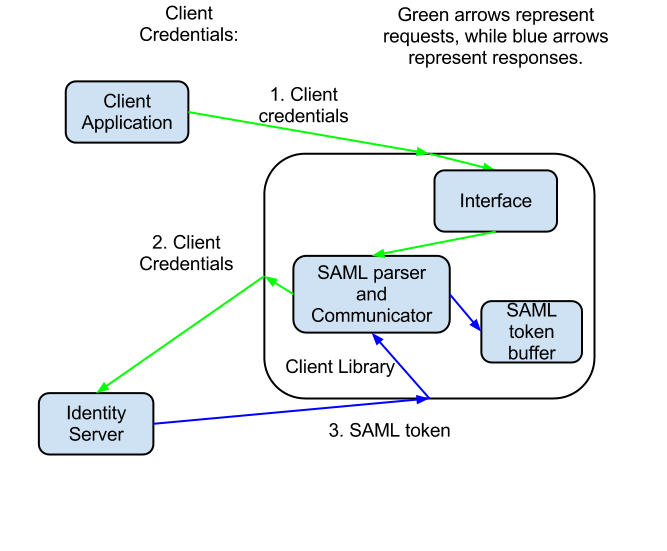
\includegraphics[width=\textwidth]{ClientCredentialsDataFlowDiagram}
        \caption{Client Credentials Flow}
        This figure describes how the client credentials are sent through the client library and through the system in general. 
        \label{fig:ClientCredentialsDataFlowDiagram}
    \end{figure}
    
    \begin{figure}[h]
        \centering
        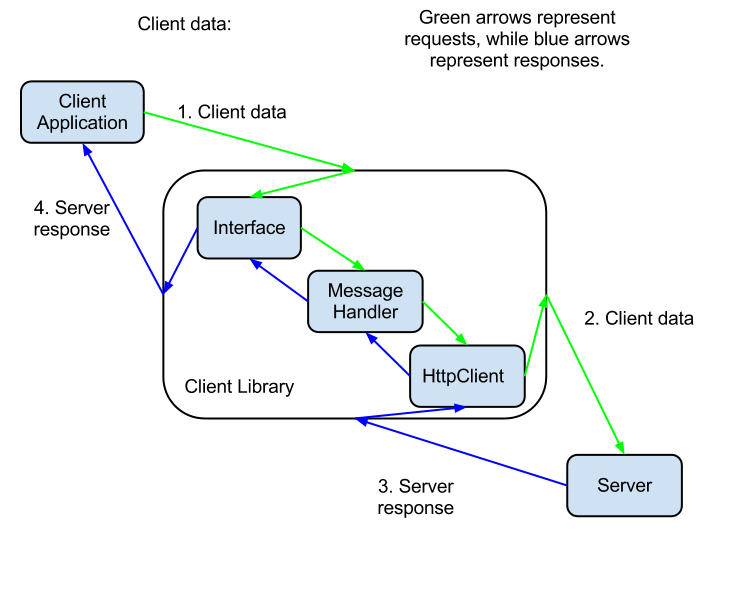
\includegraphics[width=\textwidth]{ClientDataFlowDiagram}
        \caption{Client Data Flow}
        This is the message sequence. It describes the route the individual messages takes through the system. 
        \label{fig:ClientDataFlowDiagram}
    \end{figure}
    
	\textbf{Client credentials} (Visualized in Fig:~\ref{fig:ClientCredentialsDataFlowDiagram})
		\begin{enumerate}
			\item The Client application sends credentials to the library interface
			\item The interface passes the credentials on to the token manager, through the sequencer
			\item The token manager stores the credentials in the credential storage
			\item The token manager sends the credentials to the SAML communicator in order to fetch a token
			\item The SAML communicator requests a token from the identity server
			\item The identity server sends a token to the SAML communicator
			\item The token is returned to the token manager
			\item The token manager stores the token in the credential storage
		\end{enumerate}
		\\\\	
		\textbf{Client Data} (Visualized in Fig:~\ref{fig:ClientDataFlowDiagram})
		\begin{enumerate}
			\item The client generates data and sends it to the library via API/Interface
			\item The data moves on to the sequencer and down to the message hander
			\item The message handler tells httpCore to establish a connection to the server, and the data is sent
			\item The server sends a reply that is picked up by httpCore and forwarded to the messageHandler
			\item The interface is notified of the reply
			\item The interface notifies the client that the reply is ready
		\end{enumerate}
		
	\subsubsection{Architecture}\label{client architecture}
		\begin{figure}[h]
			\centering	
			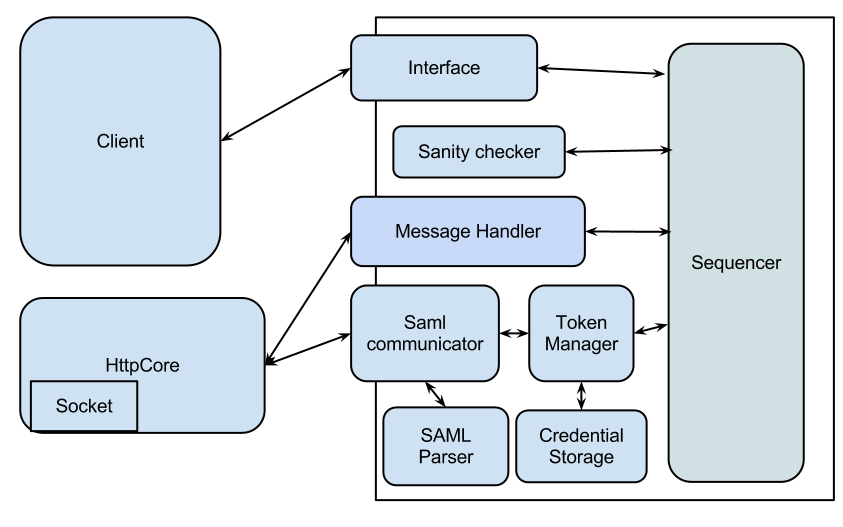
\includegraphics[width=\textwidth]{Detailedclientarchitecture}
			\caption{Detailed Client Architecture}
			This shows in detail the structure of the client library in detail. 
			\label{fig:DetailedClientArchitecture}
		\end{figure}

    All the following subparagraphs in this subsection are parts of the client library which is shown in Fig:~\ref{fig:DetailedClientArchitecture}.  \\ 
    
		\indent \textbf{Interface} \\
Known in the class diagram as “QosClient”, responsible for providing a clean and easy to use interface for the clients.
\\\\
		\indent \textbf{Sequencer} \\
The central piece of the client library. Responsible for keeping a record of all other modules in the system and communicate between them as well as making sure everything happens in the right order.
\\\\
		\indent \textbf{Sanity checker} \\
This module's single purpose is to check the credentials provided by the client for sanity, in other words make sure they conform to the rules for the credentials. It does however not verify that they are valid.
\\\\
		\indent \textbf{Token Manager} \\
This provides a nice and clean interface for the sequencer to store credentials and fetch tokens for data transmissions.
\\\\
		\indent \textbf{Saml Communicator} \\
This module will take care of the communication between the client library and the identity server.
\\\\
		\indent \textbf{Saml Parser} \\
This takes the reply from the identity server and parses it into a token object so that it can be easily used and stored.
\\\\
		\indent \textbf{Credential Storage} \\
Responsible for storing token objects as well as user supplied credentials. It's also makes sure that no token objects are returned if they are invalid or expired.

	\subsubsection{Sequence Diagrams}\label{client sequence diagrams}\\
This section contains all the sequence diagrams for the client, with descriptions for each one.
		\begin{figure}[H]
			\centering	
			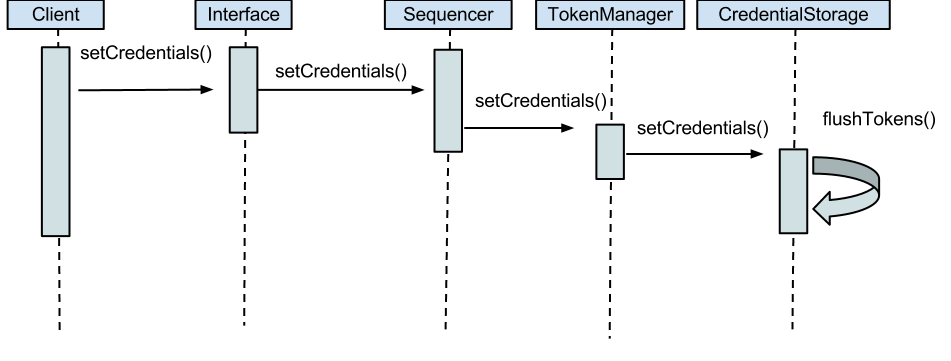
\includegraphics[width=\textwidth]{CliSeqDiaAcceptclientinfo}
			\caption{Accept client info}
			This shows how the client credentials are passed from the client, through the interface and into the credential storage.
			\label{fig:CliSeqDiaAcceptclientinfo}
		\end{figure}
		\begin{figure}[H]
			\centering	
			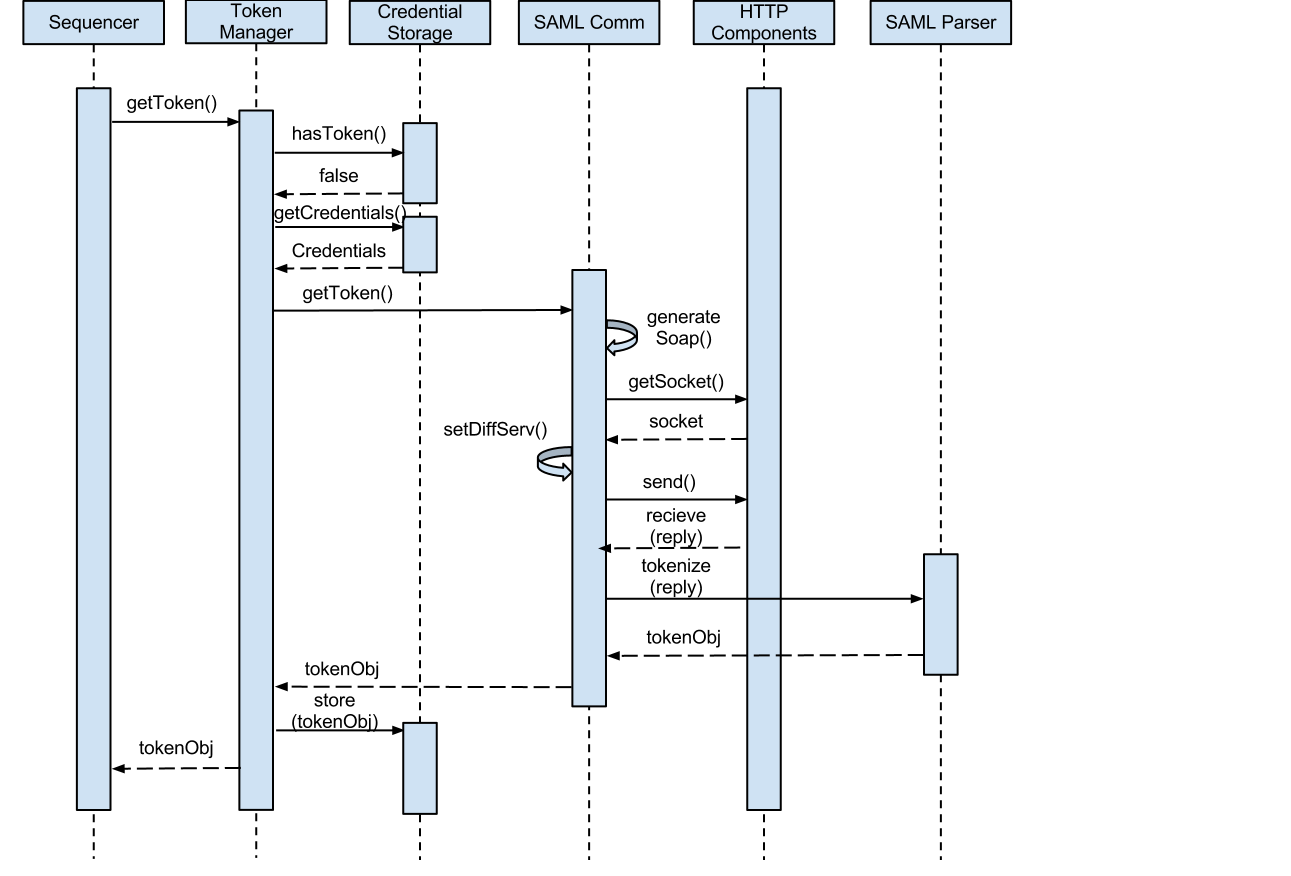
\includegraphics[scale=0.4, angle=-90]{CliSeqDiaGettingnon-storedtoken}
			\caption{Getting non-stored token}
			This shows how the client library acquires a token from an external source, and stores it, when can't find the desired token in the storage, or if the token is invalid.
			\label{fig:CliSeqDiaGettingnon-storedtoken}
		\end{figure}
		\begin{figure}[H]
			\centering	
			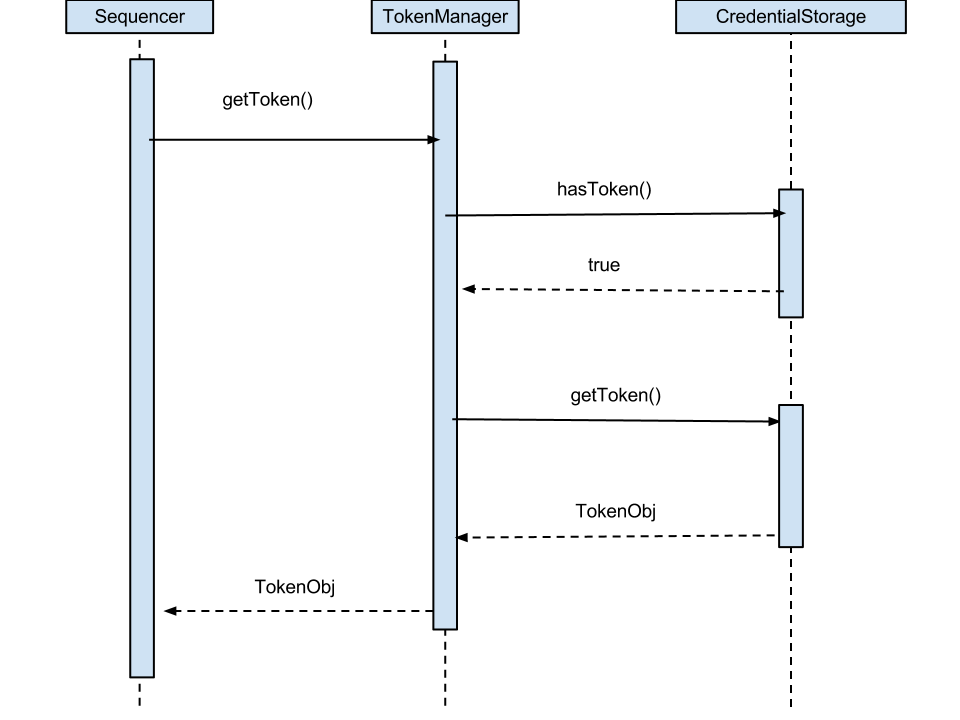
\includegraphics[scale=0.4, angle=-90]{CliSeqDiaGettingStoredToken}
			\caption{Getting stored token}
			When a token exists, we return that token instead of creating a new one. 
			\label{fig:CliSeqDiaGettingStoredToken}
		\end{figure}
		\begin{figure}[H]
			\centering	
			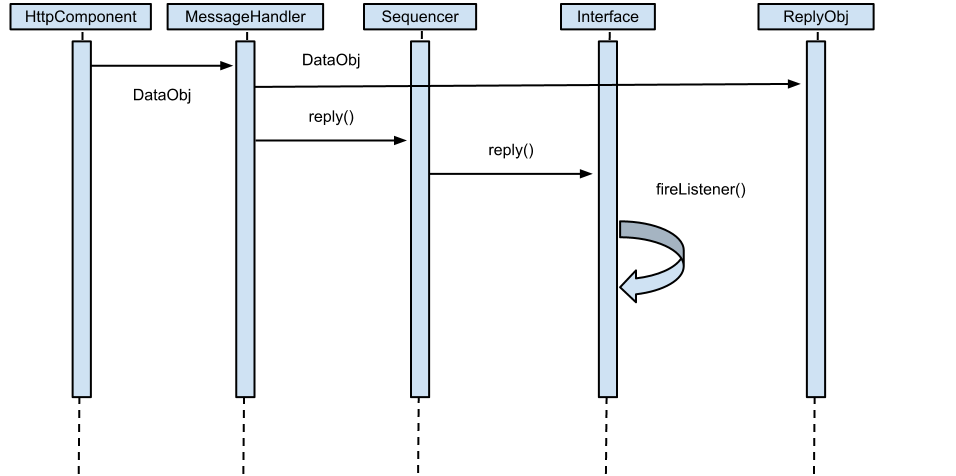
\includegraphics[scale=0.4, angle=-90]{CliSeqDiaReceivereply}
			\caption{Receive reply}
			This diagram shows how the client library receives a reply and sends it to the client. 
			\label{fig:CliSeqDiaReceivereply}
		\end{figure}
		\begin{figure}[H]
			\centering	
			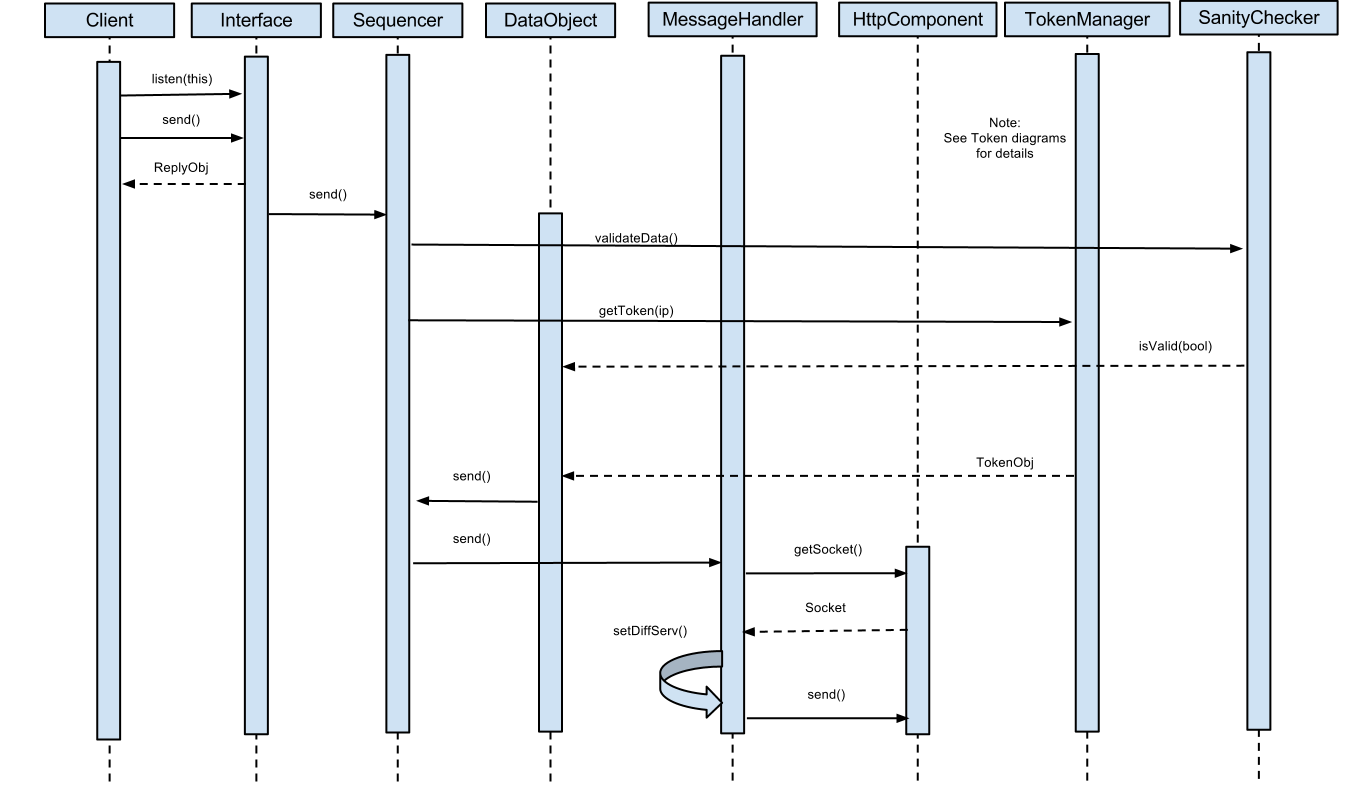
\includegraphics[scale=0.4, angle=-90]{CliSeqDiaSendData}
			\caption{Send data}
			This diagram shows how data moves through the client library, receives a token, and eventually gets sent to the server. 
			\label{fig:CliSeqDiaSendData}
		\end{figure}

		

